% summary.tex
% mainfile: perfbook.tex
% SPDX-License-Identifier: CC-BY-SA-3.0

\chapter{Looking Forward and Back}
\label{chp:Looking Forward and Back}
%
\Epigraph{History is the sum total of things that could have been avoided.}
	  {\emph{Konrad Adenauer}}

여러분은 이 책의 마지막에 도착했습니다, 수고하셨어요!
여러분의 여정이 즐겁지만 도전적이고 가치있는 것이었길 바랍니다.

여러분의 편집자와 기여자에게, 이것은 Second Edition 으로의 여정의
마지막입니다만, 함께하고자 하는 분들을 위해선 Third Edition 으로의 여정의
시작입니다.
어떻든, 이 여정을 정리해 보는게 좋겠습니다.

\Cref{chp:How To Use This Book} 은 이 책이 무엇에 관한 것인지 다루었고, 저수준
병렬 프로그래밍 외의 관심있을만한 무언가에 대한 대안도 이야기 했습니다.

\Cref{chp:Introduction} 은 병렬 프로그래밍에서의 도전 과제와 그걸 해결하는
고수준 접근법들을 다뤘습니다.
이 챕터는 또한 여전히 병렬성의 이익을 얻으면서도 이 도전과제들을 피하는
방법들을 다뤘습니다.

\iffalse

You have arrived at the end of this book, well done!
I~hope that your journey was a pleasant but challenging and worthwhile
one.

For your editor and contributors, this is the end of the journey to the
Second Edition, but for those willing to join in, it is also the start
of the journey to the Third Edition.
Either way, it is good to recap this past journey.

\Cref{chp:How To Use This Book} covered what this book is about, along
with some alternatives for those interested in something other than
low-level parallel programming.

\Cref{chp:Introduction} covered parallel-programming challenges and
high-level approaches for addressing them.
It also touched on ways of avoiding these challenges while nevertheless
still gaining most of the benefits of parallelism.

\fi

\Cref{chp:Hardware and its Habits} 는 멀티코어 하드웨어에 대한 높은 단계에서의
개론을 제공했는데, 특히 동시성 소프트웨어에 도전과제를 던져주는 것들에 대해서
그랬습니다.
이 \lcnamecref{chp:Hardware and its Habits} 는 이 도전과제들이 기인하는 것들에
대한 책임을 물었는데, 완고한 하드웨어 설계자들 보다는 많은 것이 물리 법칙에
대한 것이었습니다.
그러나, 하드웨어 설계자와 공학자들이 할 수 있을 것들도 있을 수 있으며,
\lcnamecref{chp:Hardware and its Habits} 가 그것들 약간을 다뤘습니다.
그 사이, 소프트웨어 설계자와 공학자들은 이 도전과제를 극복하기 위한 그들의
작업을 해야만 하는데, 이 책의 나머지 부분에서 이야기 된 것들입니다.

\Cref{chp:Tools of the Trade}
는 저수준 동시성 거래를 위한 도구들에 대해 짧게 알아봤습니다.
\Cref{chp:Counting} 은 이어서 그런 도구들의 사용법을---그리고, 보다 중요하게,
병렬 프로그래밍 설계 기법의 사용을--- 간단하지만 놀랍도록 어려운 동시성 카운팅
작업에 대해서---선보였습니다.
실제로 이는 매우 어려워서 여러 동시적 카운팅 알고리즘이 일반적으로 사용되고
있으며, 이것들 각각은 다른 사용처에 특화되어 있습니다.

\iffalse

\Cref{chp:Hardware and its Habits} gave a high-level overview of multicore
hardware, especially those aspects that pose challenges for concurrent
software.
This \lcnamecref{chp:Hardware and its Habits} puts the blame for these
challenges where it belongs, very much on the laws of physics and rather
less on intransigent hardware architects and designers.
However, there might be some things that hardware architects and engineers
can do, and this \lcnamecref{chp:Hardware and its Habits} discusses a few of
them.
In the meantime, software architects and engineers must do their part
to meet these challenges, as discussed in the rest of the book.

\Cref{chp:Tools of the Trade}
gave a quick overview of the tools of the low-level concurrency trade.
\Cref{chp:Counting} then demonstrated use of those tools---and, more
importantly, use of parallel-programming design techniques---on the
simple but surprisingly challenging task of concurrent counting.
So challenging, in fact, that a number of concurrent counting algorithms
are in common use, each specialized for a different use case.

\fi

\Cref{cha:Partitioning and Synchronization Design} 는 가장 중요한 병렬
프로그래밍 설계 기법인, 문제를 가능한 가장 높은 단계에서 분할하는 방법을 깊이
들여다 보았습니다.
이 \lcnamecref{cha:Partitioning and Synchronization Design} 는 또한 이 설계
공간에서의 요점 여럿을 살펴봤습니다.

\Cref{chp:Locking} 는 병렬 프로그래밍의 일꾼 (그리고 악당) 인 락킹을 상세히
알아봤습니다.
이 \lcnamecref{chp:Locking} 은 여러 종류의 락킹을 알아보고 널리 알려졌고
공격적으로 알려진 락킹의 단점들을 위한 공학적 해결법들을 선보였습니다.

\Cref{chp:Data Ownership} 는 주어진 데이터 항목과 실제 쓰레드의 연관성 의해
동기화가 제공되는 데이터 소유권의 사용을 논했습니다.
적용될 수 있는 곳이라면 이 방법은 상당한 단순성을 가지고 훌륭한 성능과 확장성을
제공합니다.

\iffalse

\Cref{cha:Partitioning and Synchronization Design} dug more deeply
into the most important parallel-programming design technique, namely
partitioning the problem at the highest possible level.
This \lcnamecref{cha:Partitioning and Synchronization Design} also
overviewed a number of points in this design space.

\Cref{chp:Locking} expounded on that parallel-programming workhorse
(and villain), locking.
This \lcnamecref{chp:Locking} covered a number of types of locking
and presented some engineering solutions to many well-known and
aggressively advertised shortcomings of locking.

\Cref{chp:Data Ownership} discussed the uses of data ownership, where
synchronization is supplied by the association of a given data item
with a specific thread.
Where it applies, this approach combines excellent performance and
scalability with profound simplicity.

\fi

\Cref{chp:Deferred Processing} 는 어떻게 약간의 지연이 놀랍도록 많은 경우에
코드를 단순화 하면서도 성능과 확장성에 거대한 개선을 가져올 수 있는지
보였습니다.
이 \lcnamecref{chp:Deferred Processing} 에서 보인 여러 메커니즘들은 CPU 캐쉬가
읽기 전용 데이터를 복사하는 기능의 장점을 취해서 빛의 속도와 원자의 크기를 크게
제한하는 물리 법칙을 회피합니다.
\Cref{chp:Data Structures} 는 길고 영광스런 병렬 프로그램의 역사를 갖는 해쉬
테이블에 집중해서 동시성 데이터 구조를 살펴봤습니다.

\Cref{chp:Validation} 은 코드 리뷰와 테스트 방법에 대해 살펴봤으며,
\cref{chp:Formal Verification} 는 정형적 검증을 살펴봤습니다.
정형적 검증/\-테스트 의 사이 어디에 여러분이 있든, 코드가 자세히 검증되지
않았다면 이는 동작하지 않습니다.
그리고 이는 동시성 코드에서는 최소 두배는 그럽니다.

\iffalse

\Cref{chp:Deferred Processing} showed how a little procrastination can
greatly improve performance and scalability, while in a surprisingly large
number of cases also simplifying the code.
A number of the mechanisms presented in this
\lcnamecref{chp:Deferred Processing}
take advantage of the ability of CPU caches to replicate read-only data,
thus sidestepping the laws of physics that cruelly limit the speed of
light and the smallness of atoms.
\Cref{chp:Data Structures} looked at concurrent data structures, with
emphasis on hash tables, which have a long and honorable history in
parallel programs.

\Cref{chp:Validation} dug into code-review and testing methods, and
\cref{chp:Formal Verification} overviewed formal verification.
Whichever side of the formal-verification/\-testing divide you might
be on, if code has not been thoroughly validated, it does not work.
And that goes at least double for concurrent code.

\fi

\Cref{chp:Putting It All Together} 는 동시성 메커니즘들을 그것들끼리 또는 다른
설계 묘수들과 조합하는 것이 병렬 프로그래머의 삶을 무척 쉽게 해줄 수 있는 여러
상황들을 보였습니다.
\Cref{sec:advsync:Advanced Synchronization} 는 고급 동기화 방법들을 알아봤는데,
lockless 프로그래밍, non-blocking synchronization, 그리고 병렬 리얼타임
컴퓨팅을 포함했습니다.
\Cref{chp:Advanced Synchronization: Memory Ordering} 는 치명적으로 중요한
주제인 메모리 순서 규칙을 알아봤는데, 여러분이 메모리 순서규칙 문제를 풀 뿐만이
아니라 그걸 완전히 회피하기 위한 기법과 도구들을 보였습니다.
\Cref{chp:Ease of Use} 는 놀랍도록 중요한 사용성이라는 주제를 짧게
알아봤습니다.

마지막이지만 절대 빼놓을 수 없는 \cref{chp:Conflicting Visions of the Future}
는 여러 충돌하는 미래에 대한 상상을 알아보았는데, CPU 기술 트렌드, 트랜잭셔널
메모리, 하드웨어 트랜잭셔널 메모리, 회귀 테스트에서의 정형적 검증의 사용,
그리고 미래의 병렬 프로그래밍이 함수형 프로그래밍 언어로 이루어질 거라는 오래된
예측을 포함했습니다.

이렇게 이 Second Edition 의 내용을 요약했습니다, 그런데 이 책은 어떻게
시작되었을까요?

\iffalse

\Cref{chp:Putting It All Together} presented a number of situations
where combining concurrency mechanisms with each other or with other
design tricks can greatly ease parallel programmers' lives.
\Cref{sec:advsync:Advanced Synchronization} looked at advanced
synchronization methods, including lockless programming, non-blocking
synchronization, and parallel real-time computing.
\Cref{chp:Advanced Synchronization: Memory Ordering} dug into the
critically important topic of memory ordering, presenting techniques
and tools to help you not only solve memory-ordering problems, but
also to avoid them completely.
\Cref{chp:Ease of Use} presented a brief overview of the surprisingly
important topic of ease of use.

Last, but definitely not least, \cref{chp:Conflicting Visions of the Future}
expounded on a number of conflicting visions of the future, including
CPU-technology trends, transactional memory, hardware transactional
memory, use of formal verification in regression testing, and the
long-standing prediction that the future of parallel programming belongs
to functional-programming languages.

But now that we have recapped the contents of this Second Edition, how did
this book get started?

\fi

Paul 의 병렬 프로그래밍 여정은 1990년대에 그가 Sequent Computer Systems, Inc 에
입사하면서 시작되었습니다.
Sequent 는 새로 고용된 엔지니어들이 그들을 멘토링하고 코드를 리뷰하고 여러
주제에 대해 풍부한 양의 조언을 주는 경험 많은 엔지니어들로 둘러싸인 작은 방에
위치하게 하는 견습 프로그램 같은걸 사용했습니다.
그 결과 이 새로 고용된 엔지니어들은 두세달 만에 생산적인 병렬 프로그래머가
되었고, 그들 중 여럿은 일이년만에 놀라운 일들을 해냈습니다.

Sequent 는 병렬성의 미스테리에서 새로운 엔지니어들을 빠르게 훈련시키는 그들의
능력이 흔하지 않음을 알아냈고, 따라서 그 회사의 병렬 프로그래밍 지혜를 기록한
짧은 책을 만들어 냈는데~\cite{SQNTParallel}, 그보다 몇년 전에 쓰여진 두개의
놀라운 논문을~\cite{Beck85,Inman85} 포함했습니다.
이미 이 미스테리에 빠져있던 사람들은 이 책과 논문들에 경의를 표했으나,
초심자들은 보통 이로부터 큰 이익을 얻기는 어려워서, 불가피하게도 그 책이나
논문들에 의해 명시적으로 금지되지 않은 고도로 창의적이고 상당히 파괴적인 에러를
만들어냈습니다.\footnote{
	``하지만 대체 왜 \emph{그걸} 한 거죠???''
	``글쎄요, 안그럴 이유가 뭐죠?''}
물론 이 상황은 Paul 이 어떤 개선된 책을 쓰는 것을 생각하기 시작하게 했으나, 이
때의 그의 노력은 내부 교육 자료와 출간된 논문들로 제한되어 있었습니다.

\iffalse

Paul's parallel-programming journey started in earnest in 1990, when
he joined Sequent Computer Systems, Inc.
Sequent used an apprenticeship-like program in which newly hired engineers
were placed in cubicles surrounded by experienced engineers, who mentored
them, reviewed their code, and gave copious quantities of advice on
a variety of topics.
The result was that these newly hired engineers became productive parallel
programmers within two or three months, and several of them were doing
ground-breaking work within a couple of years.

Sequent understood that its ability to quickly train new engineers in the
mysteries of parallelism was unusual, so it produced a slim volume that
crystalized the company's parallel-programming wisdom~\cite{SQNTParallel},
which joined a pair of groundbreaking papers that had been written a
few years earlier~\cite{Beck85,Inman85}.
People already steeped in these mysteries saluted this book and these
papers, but novices were usually unable to benefit much from them,
invariably making highly creative and quite destructive errors that
were not explicitly prohibited by either the book or the papers.\footnote{
	``But why on earth would you do \emph{that}???''
	``Well, why not?''}
This situation of course caused Paul to start thinking in terms of
writing an improved book, but his efforts during this time were limited
to internal training materials and to published papers.

\fi

1999년에 Sequent 가 IBM 에 인수되었을 때, 세계의 가장 큰 데이터베이스
인스턴스들은 Sequent 하드웨어에서 돌아가고 있었습니다.
그러나 시간은 바뀌며, 2001년에 이르러선 많은 Sequent 의 병렬 프로그래머가
리눅스 커널로 그들의 주의를 돌렸습니다.
초기의 약간의 꺼림 후, 리눅스 커널 커뮤니티는 동시성을
커뮤니티를 통한 많은 훌륭한 혁신과 개선과 함께 효과적이고 열광적으로
받아들였습니다~\cite{SilasBoydWickizer2010LinuxScales48,McKenney:2012:BEP:2414729.2414734}.
책을 써야겠다는 생각은 Paul 에게 때때로 떠올랐으나, 삶은 빠르게 흘러갔고,
따라서 그는 이 프로젝트에 진척을 내지 못하고 있었습니다.

2006년, Paul 은 리눅스 확장성에 대한 컨퍼런스에 초대받았으며, 존경받는 병렬
프로그래밍 전문가들의 패널에 마지막 질문을 던지는 특권을 얻었습니다.
Paul 은 1991년부터 2006년의 15년 동안 병렬 시스템의 가격은 집 한채 가격에서
중간대 자전거 정도까지 떨어졌음을, 그리고 다음 15년을 거쳐 2021년에 이르러서는
가격이 더욱 극적으로 떨어질 것이 분명하다고 이야기 하며 시작했습니다.
그는 또한 가격을 떨어뜨리는 것은 병렬 프로그래밍 문제를 해결하는데 상당한
친화성과 빠른 진척을 가져올 것이라고 이야기 했습니다.
이것이 그의 질문을 이끌었습니다:
``2021년에도 병렬 프로그래밍이 루틴화 되지 않는다면 그 이유는 뭘까요?''

\iffalse

By the time Sequent was acquired by IBM in 1999, many of the world's
largest database instances ran on Sequent hardware.
But times change, and by 2001 many of Sequent's parallel programmers
had shifted their focus to the Linux kernel.
After some initial reluctance, the Linux kernel community embraced
concurrency both enthusiastically and
effectively~\cite{SilasBoydWickizer2010LinuxScales48,McKenney:2012:BEP:2414729.2414734},
with many excellent innovations and improvements from throughout the
community.
The thought of writing a book occurred to Paul from time to time, but
life was flowing fast, so he made no progress on this project.

In 2006, Paul was invited to a conference on Linux scalability, and was
granted the privilege of asking the last question of panel of esteemed
parallel-programming experts.
Paul began his question by noting that in the 15~years from 1991 to 2006,
the price of a parallel system had dropped from that of a house to that
of a mid-range bicycle, and it was clear that there was much more room
for additional dramatic price decreases over the next 15~years
extending to the year 2021.
He also noted that decreasing price should result in greater familiarity
and faster progress in solving parallel-programming problems.
This led to his question:
``In the year 2021, why wouldn't parallel programming have become routine?''

\fi

첫번째 패널리스트는 그런 황당한 질문을 던지는 누구에게나 경멸을 하는 듯
보였으며, 빠르게 짧은 답을 내놓았습니다.
이는 역시 Paul 에게 짧은 답을 내놓게 했습니다.
그들은 말을 한동안 주고받았는데, 예를 들어 그 패널리스트의 짧은 답 ``데드락''
은 Paul 의 ``락 의존성 검사기'' 라는 짧은 답을 유발했습니다.

그 패널리스트는 결국 짧은 답이 떨어졌고, 임시변통으로 마지막 답을 내놓았습니다,
``당신 같은 사람들은 망치에 머리를 맞아야 한다!''

Paul 의 답은 물론 ``당신도 거기 줄서야 할겁니다!'' 였습니다.

Paul 은 그의 주의를 다음 패널리스트에게로 돌렸는데, 그는 첫번째 패널리스트에게
어느정도 동의하고 있으며 Paul 의 답변들을 처리하고 싶지 않아 하는듯 보였습니다.
따라서 그는 짧은 이도저도 아닌 말을 했습니다.
그리고 그렇게 나머지 패널들에게도 마이크가 넘어갔습니다.

\iffalse

The first panelist seemed quite disdainful of anyone who would ask such
an absurd question, and quickly responded with a soundbite answer.
To which Paul gave a soundbite response.
They went back and forth for some time, for example, the panelist's
sound-bite answer ``Deadlock'' provoked Paul's sound-bite response ``Lock
dependency checker''.

The panelist eventually ran out of soundbites, improvising a final
``People like you should be hit over the head with a hammer!''

Paul's response was of course ``You will have to get in line for that!''

Paul turned his attention to the next panelist, who seemed torn between
agreeing with the first panelist and not wishing to have to deal with
Paul's series of responses.
He therefore have a short non-committal speech.
And so it went through the rest of the panel.

\fi

여러분이 그 이름을 들어봤을지도 모르는 마지막 패널리스트, Linus Torvalds 의
차례가 올때까지는 그랬습니다.
Linus 는 3년 전 (즉, 2003) 모든 동시성에 연관된 패치들의 첫번째 버전은 보통
무척 조악했으며, 설계상의 취약점과 많은 버그를 가지고 있었다고 이야기 했습니다.
그리고 그게 받아들여지기 충분할 정도로 정리되었을 때까지도 버그들은 여전히
남아있었습니다.
Linus 는 2006년 기준으로 그때와 지금의 상황을 비교했는데, 그는 잘 설계되었고
버그는 약간만 있거나 아예 없는 동시성 연관 패치의 첫번째 버전은 그리 드물지
않다고 했습니다.
그는 이어서 \emph{만약} 도구들이 계속해서 개선된다면, \emph{아마도} 병렬
프로그래밍은 2021년에 이르러서는 일상적인 것이 될 거라고
제안했습니다.\footnote{
	2021년에 이르러 병렬 프로그래밍이 일상화 되지 않았다고 단정하려는
	사람은 \cref{chp:Introduction} 의 명구를 읽어보셔야 합니다.}

그리고는 그 컨퍼런스는 마무리 되었습니다.
Paul 은 특히나 첫번째 패널리스트가 그랬던 것과 같은 방법으로 세계를 보던
사람들을 포함한 청중들에게 둘러싸였는데 놀라지 않았습니다.
Paul 은 또한 일부 청중들은 그에게 그 질문을 던져줘 고맙다고 하는데에도 놀라지
않았습니다.
하지만, 어떤 사람이 다가와 말을 하기도 힘들정도로 흐느끼며 그의 얼굴에 눈물을
흘리며 ``고맙습니다'' 라고 하는데에는 무척 놀랐습니다.

\iffalse

Until it was the turn of the last panelist, who was someone you might have
heard of who goes by the name of Linus Torvalds.
Linus noted that three years earlier (that is, 2003), the initial version
of any concurrency-related patch was usually quite poor, having design
flaws and many bugs.
And even when it was cleaned up enough to be accepted, bugs still
remained.
Linus contrasted this with the then-current situation in 2006, in which
he said that it was not unusual for the first version of a concurrency-related
patch to be well-designed with few or even no bugs.
He then suggested that \emph{if} tools continued to improve, then \emph{maybe}
parallel programming would become routine by the year 2021.\footnote{
	Those who wish to assert that year-2021 parallel programming is
	not routine should refer to \cref{chp:Introduction}'s epigraph.}

The conference then concluded.
Paul was not surprised to be given wide berth by many audience members,
especially those who saw the world in the same way as did the first panelist.
Paul was also not surprised that a few audience members thanked him for
the question.
However, he was quite surprised when one man came up to say ``thank
you'' with tears streaming down his face, sobbing so hard that he could
barely speak.

\fi

이 사람은 Sequent 에서 수년간을 일했으며, 따라서 병렬 프로그래밍을 매우 잘
이해하고 있었습니다.
더 나아가, 그는 현재 병렬 코드를 작성하는 직업을 갖는 그룹에 할당되어
있었습니다.
그리고 그 일은 잘 진행되지 못하고 있었죠.
아시겠죠, 그들이 그의 병렬 프로그래밍에 대한 설명의 이해에 문제를 가지고 있던
게 아닙니다.

문제는 그들의 그의 말을 \emph{전혀} 들으려 하지 않고 있었다는 겁니다.

그 순간, Paul 은 ``언젠가는 책을 써야지'' 에서 ``이 책을 쓰기 위한 뭐든
해야겠다'' 라고 생각을 바꿨습니다.
Paul 은 이 남자의 이름을 기억하지 못하고 있음을 인정해야 함에 창피함을
느낍니다, 실제로 그의 이름을 알았던 적이 있긴 하다면요.

이 책은 더도 덜도 아니고 그 남자를 위한 겁니다.

\iffalse

You see, this man had worked several years at Sequent, and thus very
well understood parallel programming.
Furthermore, he was currently assigned to a group whose job it was to
write parallel code.
Which was not going well.
You see, it wasn't that they had trouble understanding his explanations
of parallel programming.

It was that they refused to listen to him \emph{at all}.
% @@@ Maybe tie back to that first panelist?

In that moment, Paul went from ``I should write a book some day'' to
``I will do whatever it takes to write this book''.
Paul is embarrassed to admit that he does not remember the man's name,
if in fact he ever knew it.

This book is nevertheless for that man.

\fi

\IfTwoColumn{
\begin{figure}
\centering
\resizebox{3in}{!}{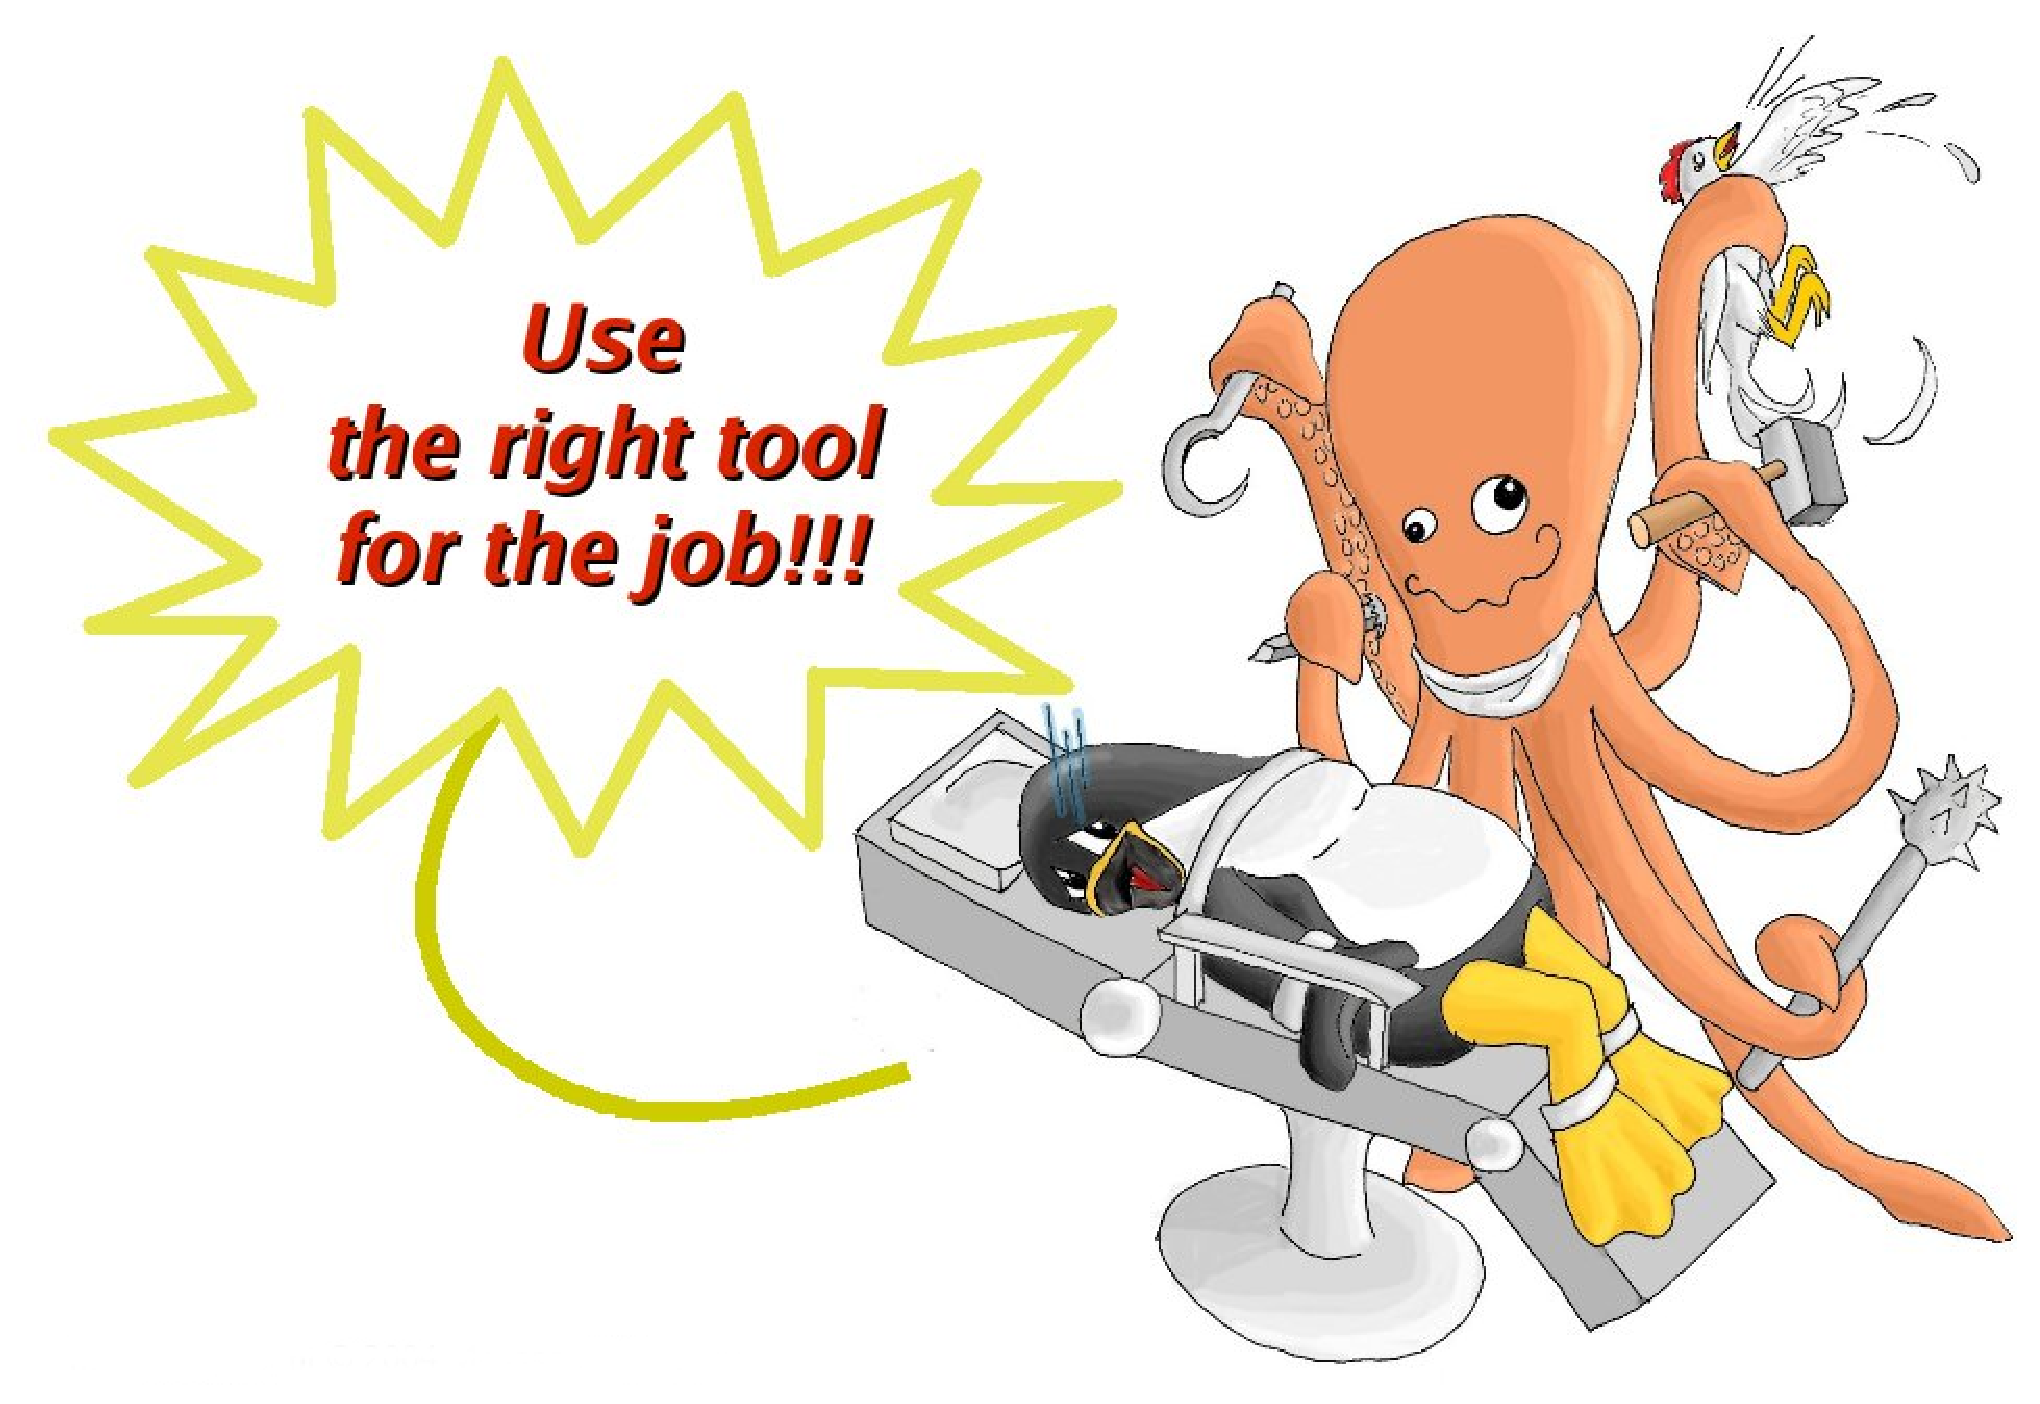
\includegraphics{cartoons/UseTheRightToolsBubble}}
\caption{The Most Important Lesson}
\ContributedBy{Figure}{fig:summary:The Most Important Lesson}{Melissa Broussard}
\end{figure}
}{
\begin{figure}[H]
\centering
\resizebox{3in}{!}{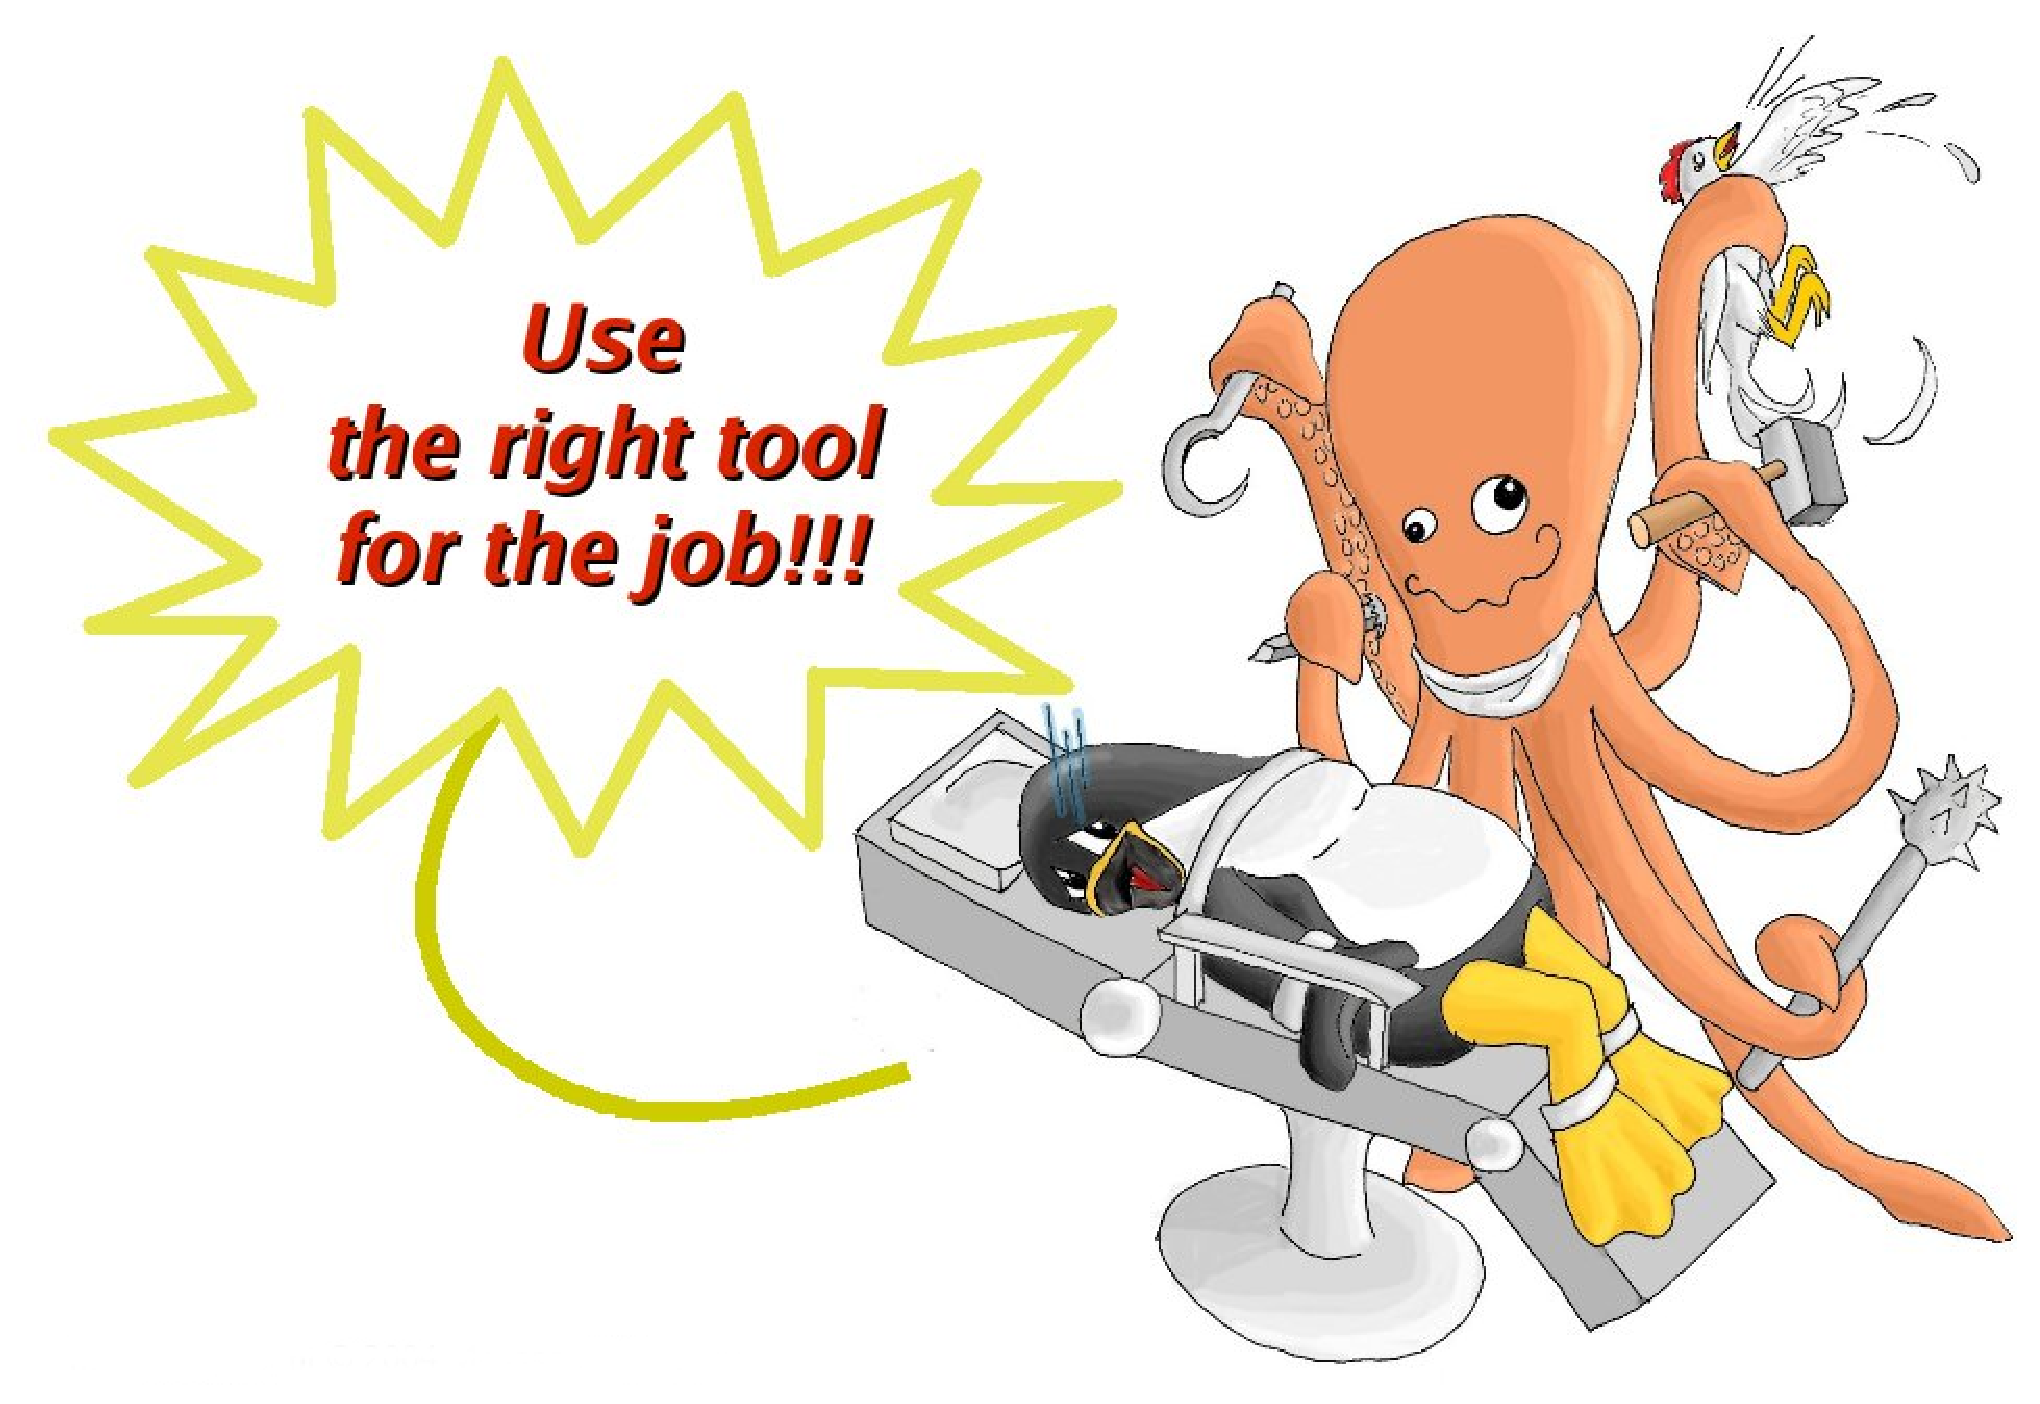
\includegraphics{cartoons/UseTheRightToolsBubble}}
\caption{The Most Important Lesson}
\ContributedBy{Figure}{fig:summary:The Most Important Lesson}{Melissa Broussard}
\end{figure}
}

그리고 이 책은 또한 그들의 기술 목록에 저수준 동시성을 추가하고 싶은 모두를
위한 것이기도 합니다.
여러분이 이 책에서 그 외에는 어떤 것도 기억하지 못한다면,
\cref{fig:summary:The Most Important Lesson} 의 교훈을 생각하십시오.

나머지 우리들을 위해선, 누군가가 우리에게 어려운 문제를 어떻게 해결하는지
보여주려 한다면, 우린 최소한 듣기를 하는 선행을 베풀 수 있을 겁니다.

\iffalse

And this book is also for everyone else who would like to add low-level
concurrency to their skillset.
If you remember nothing else from this book, let it be the lesson of
\cref{fig:summary:The Most Important Lesson}.

For the rest of us, when someone tries to show us how to solve a pressing
problem, perhaps we should do them the courtesy of at least listening!

\fi

% @@@	Perhaps add discussion of the changes in Linux development
% @@@	from 2003-2006.
% @@@	Maybe also history of book back in 2004-2006.
